\chapter{Experiences}\label{chapter:experiences}

Given the relatively nascent status of the Cerebras WSE-2 accelerator and its limited adoption, this chapter aims to succinctly outline our experiences concerning the available tools, workflow, and programming model, with the anticipation that future endeavors may benefit from these insights. We organize this chapter into four sections, beginning with an exploration of the Cerebras WSE-2 and proceeding to discuss the workflow involved in developing for the device.

\section{Cerebras WSE-2}

The Cerebras WSE-2 is still in its infancy regarding development. It offers a robust programming language and an SDK\footnote{https://sdk.cerebras.net/} for device development, along with comprehensive documentation to support beginners in their work with the device. The Multiple Instruction, Multiple Data (MIMD) programming paradigm employed differs from conventional paradigms in High-Performance Computing (HPC). Our endeavor to implement Matrix Profiling on the Cerebras represents a pioneering effort and is ripe for refinement, although we have yet to explore the full extent of the device's capabilities.

\section{Workflow}

The workflow for the Cerebras WSE-2 resembles that of working on an embedded device. The compiler\footnote{https://sdk.cerebras.net/csl/csl-compiler} produces binaries that must be transferred to the Simulator/Device. However, the SDK is still in its nascent stage and lacks certain utilities, such as facilitating large data transfers to the wafer. Nonetheless, it includes multiple examples, such as the \texttt{GEMV} implementation\footnote{https://sdk.cerebras.net/csl/code-examples/benchmark-gemv-checkerboard}, which serve as valuable points of reference. Subsequently, we developed a \texttt{Wrapper Application} enabling flexible execution of time series, result verification, and data collection from the device.

\subsection{Transitioning from Simulator to Device}

The Cerebras SDK provides clear guidelines on transitioning from the Simulator\footnote{https://sdk.cerebras.net/appliance-mode} to the device, making the switch seamless. Notably, the device imposes limitations on the number of Processing Elements (PEs) allocatable at any given time due to bandwidth-constrained memory transfer commands via a Remote Procedure Call (RPC) backend. This constraint is expected to be addressed in the forthcoming CSSoft 2.2 software release for WSC, which will streamline transitions between simulator programs and wafer-scale clusters. It will include the ability to pre-stage data on one of the cluster's worker nodes, thereby circumventing the need for gRPC transfers.

\section{Build Process}

Build times for the simulator are expedited since it directly invokes the \texttt{cslc} compiler. Conversely, device compilation is managed by the SLURM instance managing the Wafer cluster\footnote{https://docs.cerebras.net/en/latest/wsc/general/slurm-integration.html\#slurm-integration} in EIDF and is abstracted from the user. Our program's execution times on the device are depicted in Figure \ref{fig:average_execution_time}.

\begin{figure}[h!]
    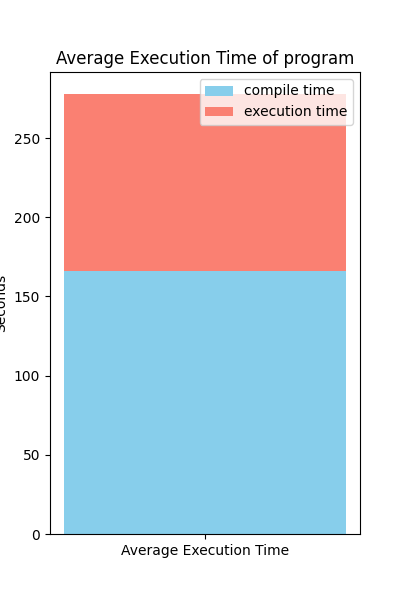
\includegraphics[scale=0.45]{average_execution_time.png}
    \centering
    \caption{\textit{Average Execution Times} of a Matrix Profiling program on the Cerebras}
    \label{fig:average_execution_time}
\end{figure}

We initially tested our implementation on the simulator using small inputs. Once an acceptable error rate in the matrix profile was achieved, we ported the application to run on the wafer cluster setup at EDIF and the process was seamless.
